\chapter{Návrh}
V~rámci této kapitoly bude nejprve vybrána aplikace, která bude použita k~otestování použitelnosti frameworku Compose Multiplatform a následně
bude tato aplikace navržena tak, aby splnila veškeré vytyčené cíle z~úvodní sekce \textit{Cíle práce \ref{goals}}.

Po vybrání typu aplikace následuje sekce věnující se detekci případů užití. Ty je zejména vhodné specifikovat proto, aby bylo zřejmé jací 
uživatelé budou danou aplikaci používat. Dalším aspektem je výběr platforem, pro které bude následně aplikace implementována. %pohledu na jakých zařízení případně platformách ji budou využívat. 
Zároveň bude hledáno vhodné skloubení případů užití s~grafickou podobou UI tak, aby nejčastějšímu uživateli bylo možné splnit cíle, s~co nejmenší dávkou úsilí. 
To je totiž pro správný návrh UI klíčové. 
%což obecně vede k intenzivnějšímu používaní a oblibě aplikace.

Další fáze návrhu je věnována vytyčení funkčních požadavků, pomocí kterých je jasně specifikováno, jakými funkcionalitami by měla výsledná 
aplikace disponovat. 

Dále je v~rámci této kapitoly navržena architektura aplikace, která je pro následné navržení a správné fungování UI nezbytná. Sekce \textit{Návrh architektury} se tedy věnuje rozebrání aktuálně uplatňovaným principů při návrhu správně architektury pro mobilní zařízení a následnému detailnímu
rozebrání jednotlivých vrstev navržené architektury.

V~poslední části návrhu je přistoupeno k~samotnému návrhu uživatelského rozhraní aplikace a to nejprve za použití takzvaných drátěných modelů. V dalším kroku je přistoupeno k návrhu design systému a nakonec k~návrhu konečné podoby UI včetně grafických prvků.


\section{Výběr aplikace}
Základním požadavkem bylo vybrat takovou aplikaci, ve které by bylo možné použít velké množství různých komponent, jejichž funkčnost by následně mohla být otestována
na různých platformách.
Mezi další požadavky při výběru aplikace patřilo zaměření se na nějakou část UI, která je z pohledu multiplatformní implementace složitější a takovou část do aplikace naimplementovat.

Z~těchto důvodů byla k~implementaci vybrána aplikace sloužící pro občany měst či obcí, která kombinuje veškeré funkční požadavky plynoucí ze zadání.

Tato aplikace by sloužila občanům k~získání informací o~aktuálních novinkách, pořádaných akcích nebo například nabízela možnost vyhledat a zaplatit parkovné.

\medskip

Na základě tohoto popisu je již zřejmé, že těmto požadavkům nejlépe vyhoví mobilní aplikace, která bude použitelná na aktuálně nejrozšířenějších
mobilních platformách, kterými jsou Android a iOS \cite{iosAndroid}. 

% TODO rozsirit uvodni popis aplikace provest analyzu co by takova apk mela obsahovat

Pro potvrzení této hypotézy byly specifikovány následující případy užití.

\section{Případy užití}
Případy užití  (zkráceně UC - z~anglického \uv{use case}) jsou scénáře popisující, jakým způsobem by případní uživatelé aplikace mohli využívat určité funkce nebo
vlastnosti aplikace k~dosažení svých cílů. \cite{figmaUseCase} Tyto scénáře zachycují interakce mezi uživatelem a systémem a popisují, jak systém reaguje na určité vstupy od 
uživatele. Zároveň popisují jakou zpětnou vazbu uživatel na základě provedených vstupů od systému dostává.

\medskip

Každý případ užití obvykle obsahuje následující prvky:

\begin{itemize}
  \item \textbf{Název:} Stručný název, který popisuje, čeho chce uživatel dosáhnout.
  \item \textbf{Aktér:} Uživatel nebo systém, který spouští případ užití.
  \item \textbf{Popis:} Podrobný popis scénáře, který obsahuje kroky, které uživatel vykonává a odpovědi systému na tyto kroky.
  %\item Předpoklady: Podmínky nebo situace, které musí být splněny, aby mohl být případ užití spuštěn.
  %\item Výsledek: Očekávaný výsledek akce provedené uživatelem.
\end{itemize}

\myparagraph{Aktéři}
Hlavními aktéry systému jsou především občané příslušného města, kteří budou aplikaci využívat za účelem splnění cílů 
zmíněných v~rámci této kapitoly. 
Dalším aktérem tohoto systému je informační systém (IS) města, který aplikaci poskytuje potřebná data. 

\medskip
\textit{Pozn. Následující případy užití jsou pro jednoduchost popsány pouze z~pohledu občanů města a z~toho důvodu 
explicitně nespecifikují aktéra, jehož se daný případ užití týká.
}

%TODO jaci uzivatel budou aplikaci použivat

\myparagraph{UC1 Získání aktuálních novinek}
Získání přístupu k~aktuálním novinkám a důležitým oznámením. 
ze svého města nebo obce. %Tato funkce umožní občanům zůstat informováni o dění ve svém okolí.

\begin{enumerate}
  \item Systém uživateli poskytne seznam aktualit načtený z~webových stránek města a dalších informačních zdrojů.
  \item Uživatel si vybere aktualitu, která ho zaujme.
  \item Systém uživateli vrátí detail vybrané aktuality obsahující její název, obsah, datum vytvoření, obrázek a případně odkazy na další zdroje.
\end{enumerate}

\myparagraph{UC2 Získání aktuálních událostí} 
Získání přehledu o~aktuálně připravovaných akcích, událostech a kulturních 
aktivitách ve vybraném městě nebo obci. 

\begin{enumerate}
  \item Systém uživateli poskytne aktuální seznam událostí z~webových stránek města, divadel, kin a dalších informačních zdrojů.
  \item Uživatel si vybere událost, která ho zaujme.
  \item Systém uživateli poskytne detail vybrané události obsahující její název, datum konání, popis, místo konání obrázek a případně odkazy na další zdroje.
\end{enumerate}

\myparagraph{UC3 Získání událostí za základě času}
Filtrování zobrazených událostí na základě data konání jednotlivých událostí.

\begin{enumerate}
  \item Systém uživateli poskytne seznam událostí z~webových stránek města, divadel, kin a dalších informačních zdrojů, které 
  jsou rozděleny na základě kategorií jako například kino, divadlo, hudba atd..
  \item Uživatel si vybere konkrétní den nebo časový rozsah, pro který chce zobrazit konané události.
  \item Systém uživateli poskytne seznam událostí konaných ve vybraný den (případně vybraný časový rozsah) a tyto události zároveň
  rozdělí podle příslušných kategorií.
\end{enumerate}

\myparagraph{UC4 Získání kontaktů na místní úřady}
Získání kontaktů na místní úřady nebo správní orgány. 

\begin{enumerate}
  \item Systém uživateli poskytne seznam městských institucí.
  \item Uživatel vybere konkrétní instituci, pro kterou chce zobrazit detailní informace.
  \item Systém vrátí podrobné informace o~vybrané instituci.  
\end{enumerate}

\myparagraph{UC5 Nahlášení závady ve městě}
Možnost nahlášení závady na území města.

\begin{enumerate}
  \item Systém uživateli poskytne formulář k~vyplnění. % vázaný k nějaké z městských institucí.
  \item Uživatel vyplní název závady, nahraje fotografii závady, vyplní místo, kde se závada nachází, vybere kategorii závad do, které závada spadá a 
  záznam o~závadě odešle.
  \item Systém závadu odešle příslušnému orgánu a uživateli vrátí informaci o~jejím zaslání.
  
  %\item TODO rozdvojka spatne dobre vyplnene
\end{enumerate}

\myparagraph{UC6 Propojení se sociálními kanály města}
Možnost konzumovat aktuální novinky prostřednictvím videí z~městského YouTube kanálu nebo prostřednictvím sociální sítě Facebook.

\begin{enumerate}
  \item Systém uživateli poskytne městem používané sociální sítě.
  \item Uživatel zvolí požadovanou sociální síť.
  \item Systém uživatele přesměruje na požadovanou sociální síť.
\end{enumerate}

\myparagraph{UC7 Vyhledání parkovacích zón}
Možnost jednoduše vyhledat veškeré parkovací zóny ve městě včetně informace o~provozní době a ceníku parkovací zóny.

\begin{enumerate}
  \item Systém uživateli poskytne mapu parkovacích zón.
  \item Uživatel vybere parkovací zónu, pro kterou požaduje zobrazit detailní informace.
  \item Systém uživateli vrátí detailní informace týkající se vybrané parkovací zóny.
\end{enumerate}

\myparagraph{UC8 Platba parkovného} % podTask UC7
Možnost rychle zaplatit poplatek za parkování.

\begin{enumerate}
  \item Systém uživateli zobrazí mapu parkovacích zón v~příslušném městě.
  \item Uživatel vybere parkovací zónu, pro kterou si přeje zaplatit poplatek za parkování.
  \item Systém uživateli vrátí detailní informace týkající se vybrané parkovací zóny.
  \item Uživatel v~detailu vybrané parkovací zóny vybere akci \uv{zaplatit poplatek za parkování}.
  \item Systém uživatele přesměruje na platební systém používaný daným městem pro platbu parkovného s~předvyplněnou informací o~vybrané parkovací zóně.
\end{enumerate}

\myparagraph{UC9 Získání aktuální dopravní situace}
Možnost rychle získat přehled o~aktuální dopraní situaci ve městě.
\begin{enumerate}
  \item Systém uživateli zobrazí mapu vytíženosti jednotlivých silnic v~rámci města.
  \item Uživatel tuto informaci zpracuje.
\end{enumerate}

Pro dotvoření představy o~tom, jak jsou spolu jednotlivé případy užití navzájem propojeny, slouží obrázek \ref{fig:use_case_diagram}, který zároveň 
obsahuje i typy uživatelů pracujících s~navrženou aplikací.

%Co se týče vzájemných vazeb, tak zde je věno

\begin{figure}[H]
  \centering
  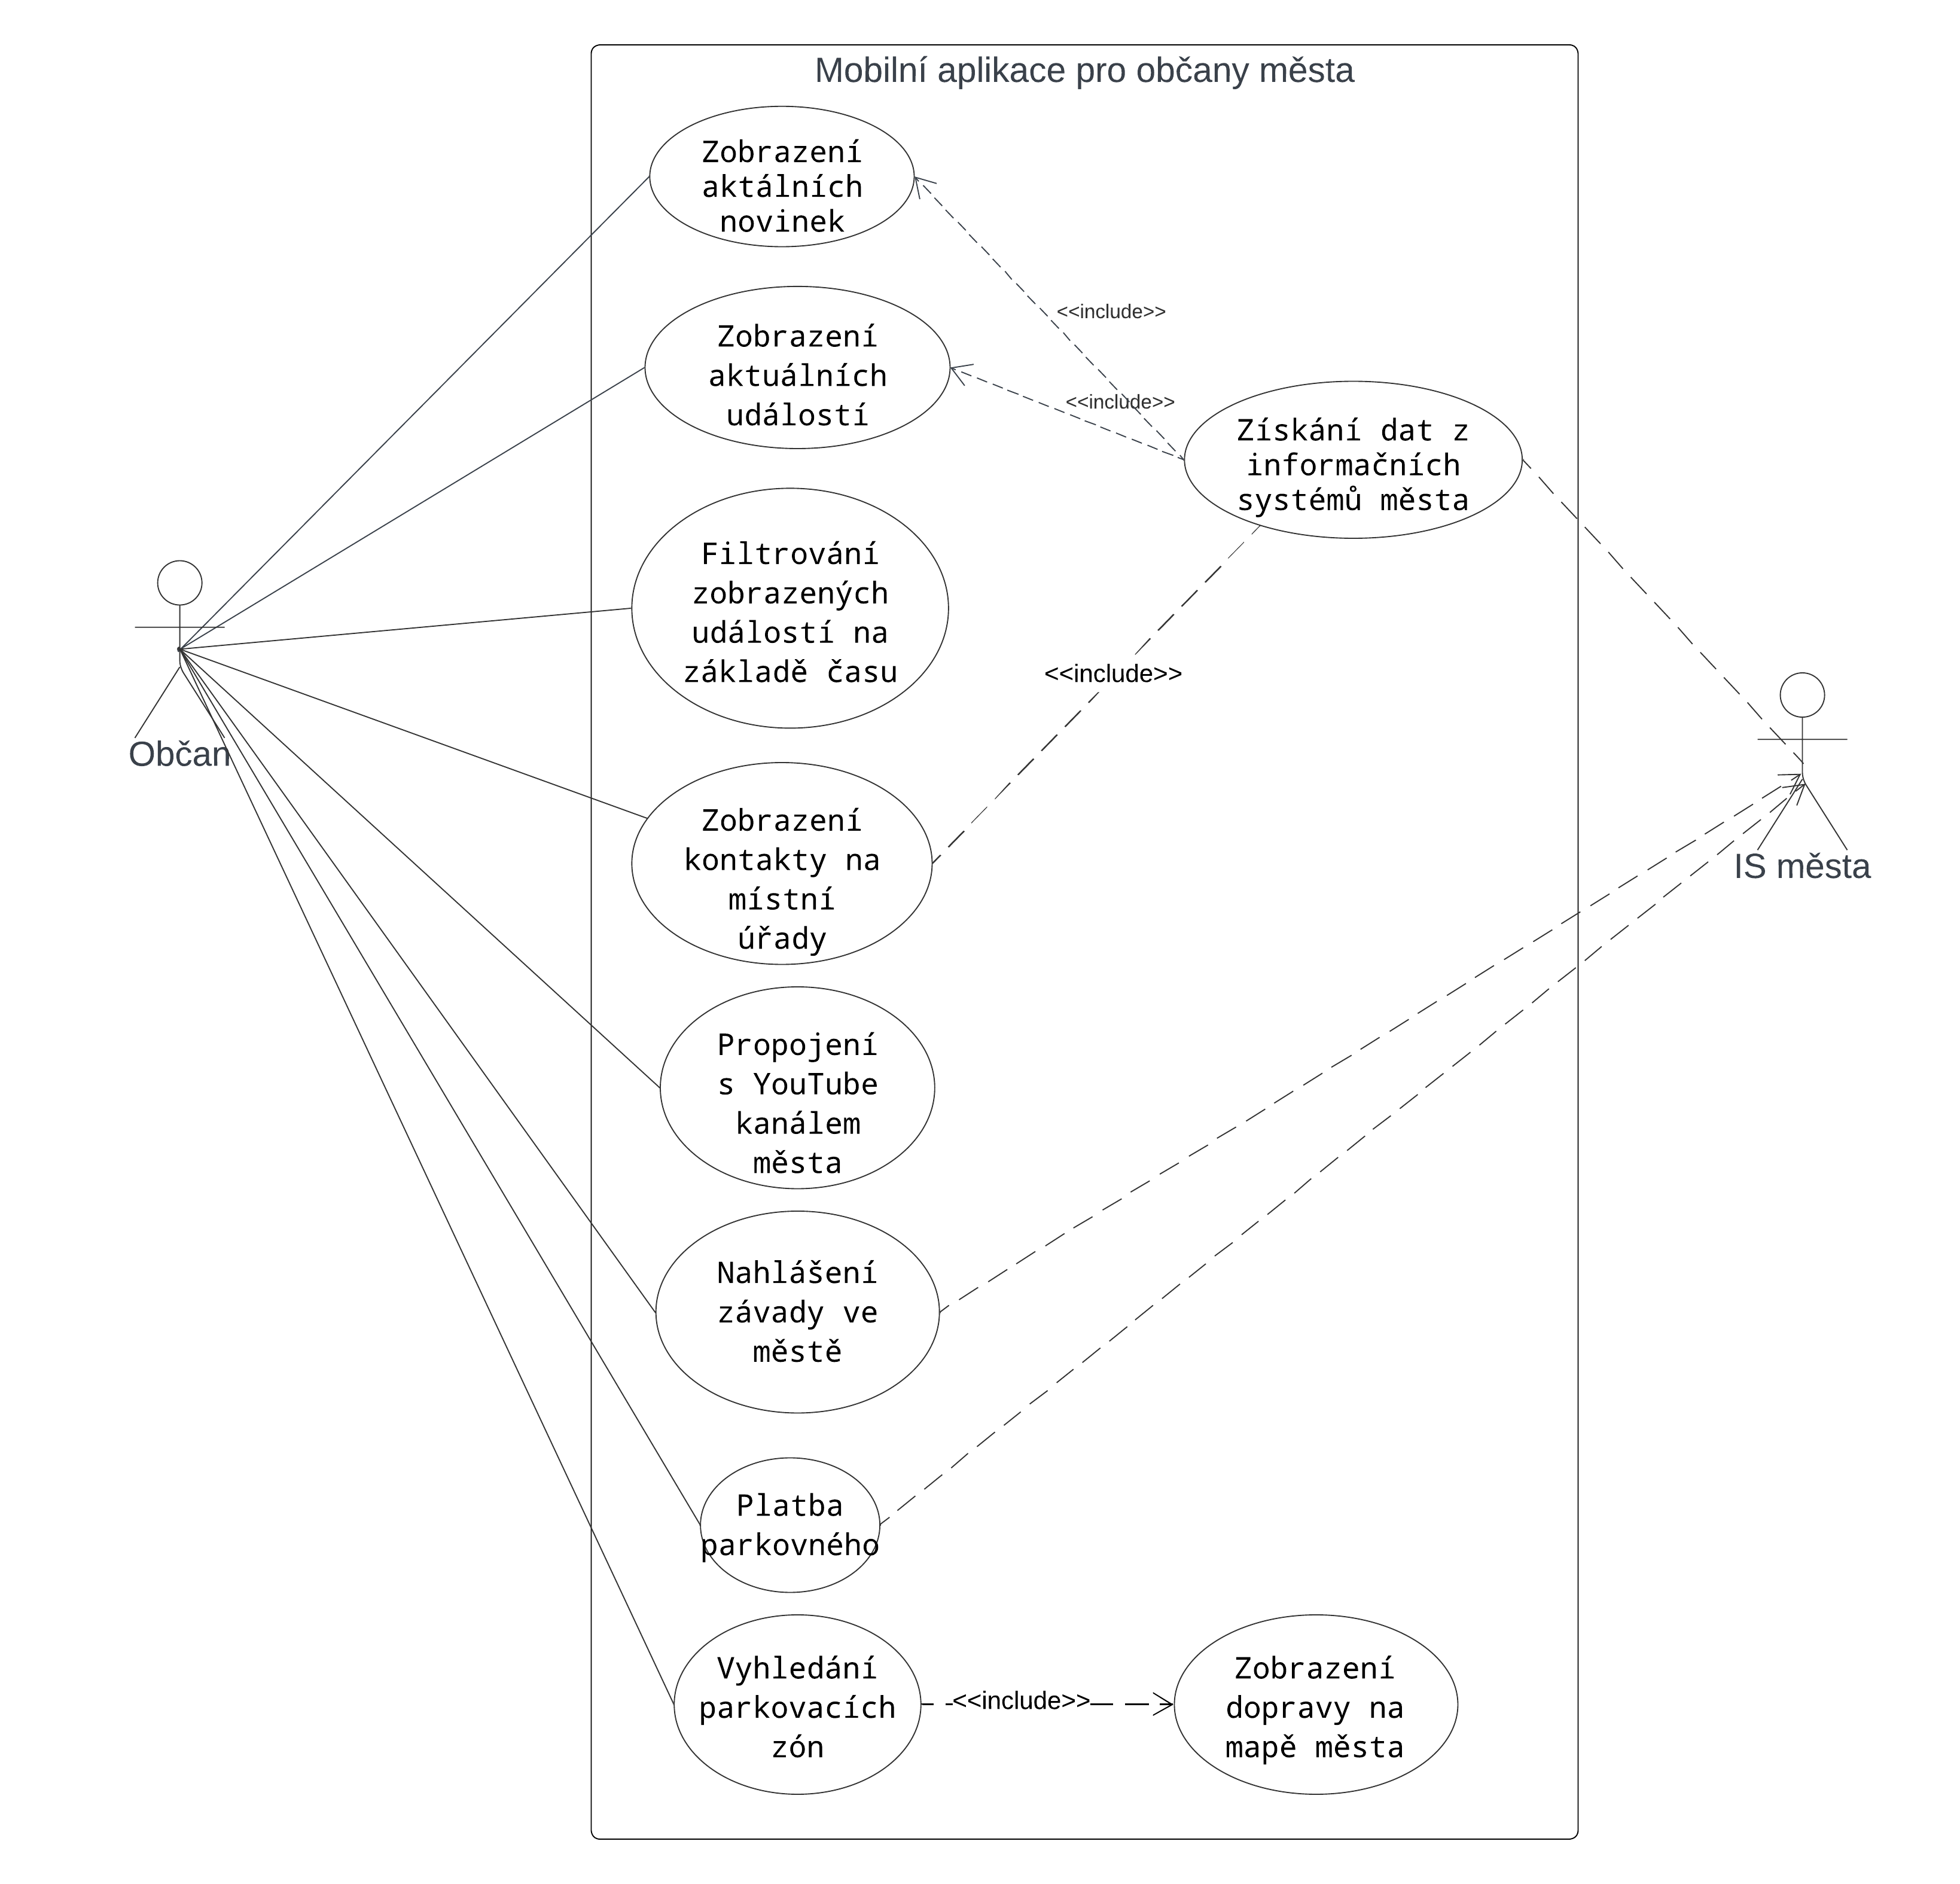
\includegraphics[width=.99\textwidth]{Use case diagram.png}
  \caption{Diagram případů užití}
  \label{fig:use_case_diagram}
\end{figure}

\bigskip

Případy užití jsou klíčovým nástrojem pro pochopení potřeb uživatelů a návrhu funkcionalit aplikace tak, aby co nejlépe odpovídaly těmto potřebám. 
Jsou také důležitým zdrojem pro testování a validaci funkčnosti aplikace, jelikož lze díky nim jednoduše ověřit, zda systém správně reaguje na očekávané 
uživatelské interakce. Podrobněji se tomuto tématu věnuje poslední kapitola \textit{Testování \ref{testsSection}} ,v~rámci které byly případy užití
použity jako základ k~tvorbě UI testů.


%koncové testování celé aplikace čehož je využito  v kapitole .

\section{Specifikace požadavků}
Na základě případů užití sepsaných v~předchozí sekci, je nyní možné sepsat konkrétní požadavky na vybranou aplikaci.
Pro konkretizaci těchto požadavků byla použita specifikace na základě funkčních a nefunkčních požadavků, která je součástí \textit{ISO/IEC/IEEE 29148:2018}\cite{iso},
jenž popisuje proces vývoje softwarových produktů.

\subsection{Funkční požadavky}
Funkční požadavky (zkráceně FR - z~anglického \uv{functional requirement}) definují konkrétní funkce a chování systému z~pohledu uživatele. 
Obecně se dá říci, že specifikují, co má systém dělat, jaké úkoly má provádět a jaké operace musí uživatelům umožňovat. \cite{functionalReq}

Pro jednodušší rozhodnutí o tom, jaká funkcionalita má být při realizaci systému implementována nejdříve a s co největším důrazem
 na kvalitu provedení, je u jednotlivých požadavků zmíněno, jakou prioritu mají a jak složité jsou na implementaci.

Obě tyto hodnoty jsou hodnoceny na stupnici 1 až 5, kde 5 je největší priorita (případně složitost) a 1 je nejmenší.


%Funkční požadavky popisují očekávané výsledky a chování systému v různých situacích.

%které zajistí, že bude aplikace pro občany měst či obcí 
%užitečná, efektivní a snadno použitelná.

\myparagraph{FR1 Zobrazení aktualit a událostí}
Systém bude přehledně zobrazovat seznamy aktualit a událostí v~daném městě, včetně jejich detailních informací, jako jsou názvy jednotlivých
událostí a novinek, časy vydání aktualit (případně datová rozmezí konání událostí) a příslušné popisy těchto událostí a novinek.

\begin{itemize}
  \item \textit{Priorita: 5}
  \item \textit{Složitost: 4}
\end{itemize}

% \myparagraph{FR4 Synchronizace s IS města}
% Systém bude synchronizován s informačními systémy města tak, aby vždy kdy je to možné zobrazoval aktuální data.
% Zároveň bude uživatele informovat o stavu synchronizace.

% \begin{itemize}
%   \item \textit{Priorita: 3}
%   \item \textit{Složitost: 2}
% \end{itemize}

\myparagraph{FR2 Filtorvání událostí}
Systém bude filtrovat konané události v~daném městě podle data jednotlivých událostí a tyto události zároveň přehledně rozřadí do patřičných
kategorií, jako například \textit{Kino}, \textit{Divadlo}, \textit{Celodenní akce} \textit{Akce pro děti} a další.

\begin{itemize}
  \item \textit{Priorita: 4}
  \item \textit{Složitost: 4}
\end{itemize}

\myparagraph{FR3 Propojení s~komunikačními kanály města}
Systém poskytne uživateli propojení s~aktuálně používanými sociálními sítěmi města buďto v~podobě odkázání na webové stránky 
dané sociální sítě nebo rovnou pomocí otevření profilu města v~aplikaci vybrané sociální sítě.  

\begin{itemize}
  \item \textit{Priorita: 3}
  \item \textit{Složitost: 1}
\end{itemize}

\myparagraph{FR4 Zpracovávat nahlášené závady}
Systém uživateli poskytne přehledný formulář pro zaslání závady do informačního systému města, do kterého je 
možné vepsat název, popis, druh závady a případně její fotografii. Tuto závadu zároveň patřičně zpracuje a zašle do IS města.

\begin{itemize}
  \item \textit{Priorita: 1}
  \item \textit{Složitost: 3}
\end{itemize}

\myparagraph{FR5 Zobrazit kontakty na místní úřady}
Pomocí systému bude možné zobrazit aktuální kontakty na místní úřady, jejich pracovní dobu a konkrétní otevírací hodiny pro každý z místních úřadů.

\begin{itemize}
  \item \textit{Priorita: 2}
  \item \textit{Složitost: 2}
\end{itemize}

\myparagraph{FR6 Správa parkovacích zón}
Pomocí systému bude možné zobrazit detailní informace o~parkovacích zónách jako je provozní doba nebo výše parkovacích 
poplatků a současně tyto parkovací poplatky pro vybranou zónu zaplatit.
\begin{itemize}
  \item \textit{Priorita: 3}
  \item \textit{Složitost: 5}
\end{itemize}

\myparagraph{FR7 Zobrazení dopravy na mapě města}
Pomocí systému bude možné jednoduše a rychle zobrazit aktuální vytíženost silnic ve městě pomocí intuitivní překryvné vrstvy mapových podkladů.

\begin{itemize}
  \item \textit{Priorita: 2}
  \item \textit{Složitost: 2}
\end{itemize}

\section*{Pokrytí případů užití} 
Pro ověření a názornou ukázku, že takto sepsané funkční požadavky pokrývají všechny případy užití, 
byla vytvořena následující tabulka pokrytí. \ref{table:tabulkaPokryti}

\bigskip

\begin{table}[H]
  \centering
  \begin{tabular}{|l|c|c|c|c|c|c|c|}
  \hline
  %\multicolumn{9}{|c|}{Functional Requirements} \\ \hline
       & FR1     & FR2     & FR3     & FR4     & FR5     & FR6     & FR7  \\ \hline
  UC1  & $\ast$ &        &        &        &        &        &         \\ \hline
  UC2  & $\ast$ &        &        &        &        &        &         \\ \hline
  UC3  &        & $\ast$ &        &        &        &        &         \\ \hline
  UC4  &        &        &        &        & $\ast$ &        &         \\ \hline
  UC5  &        &        &        & $\ast$ &        &        &         \\ \hline
  UC6  &        &        & $\ast$ &        &        &        &         \\ \hline
  UC7  &        &        &        &        &        & $\ast$ &         \\ \hline
  UC8  &        &        &        &        &        & $\ast$ &         \\ \hline
  UC9  &        &        &        &        &        &        &  $\ast$ \\ \hline
  \end{tabular}
  \caption{Pokrytí případů užití funkčními požadavky aplikace}
  \label{table:tabulkaPokryti}
\end{table}


\subsection{Nefunkční požadavky}
Nefunkční požadavky (zkráceně NFR - z~anglického \uv{Non-functional requirement}) se oproti funkčním požadavkům nezaměřují na funkčnost samotného produktu (\uv{co má systém dělat}),
ale spíše na jeho vlastnosti (\uv{jaký má být}) z~pohledu
výkonu, spolehlivosti, bezpečnosti, uživatelské přívětivosti a dalších aspektů, které nepřímo ovlivňují uživatelský zážitek a kvalitu systému. \cite{functionalReq}
Tyto požadavky jsou z~tohoto důvodu často spojeny s~technickými a provozními charakteristikami systému.

\myparagraph{NFR Multiplatformnost}
Systém by měl být dostupný alespoň na mobilních platformách.

%aby tak aby uživatele měli potřebné informaci ihned po ruce

%a pro zaruceni multiplatformnosti bude pouzit framework Compose Multiplatform a KMP

\myparagraph{NFR1 Rozšiřitelnost}
Systém by měl být rozšiřitelný na ostatní podporované platformy. % a nove funkce

\myparagraph{NFR2 Offline dostupnost}
Systém by měl správně fungovat i v~případě, že není připojen k~internetu.

\myparagraph{NFR3 Přístupnost}
Systém by měl být přizpůsoben širokému spektru lidí - například zrakově postiženým.
  

\section{Architektura aplikace}
Navržená architektura se z~velké části drží architektonických principů shrnutých v~Android dokumentaci.

%TODO %možné architektury pro vývoj mobilních aplikací

\subsection*{Důležité principy}

\myparagraph{Separation of concerns}
Separation of concerns je princip návrhu softwaru, který popisuje důležitost oddělení různých funkcionalit do samostatných, dobře definovaných a izolovaných částí. \cite{sapSep}
Hlavním cílem tohoto principu je zlepšit modularitu, udržitelnost, znovupoužitelnost a spravovatelnost kódu.

Princip oddělení zájmů (odpovědností) rozděluje systém na jednotlivé komponenty nebo moduly, přičemž každý z~nich se zabývá jednou konkrétní 
oblastí funkcionality. Každá část systému má jasně definované rozhraní, které umožňuje interakci s~ostatními částmi. \cite{sapSep}
Tímto způsobem lze snadněji spravovat a udržovat kód, protože změny v~jedné části systému nemusí mít nežádoucí dopady na ostatní části.

Příklady oddělení zájmů zahrnují oddělení prezentační vrstvy od logiky aplikace (Model-View-Controller), oddělení datového přístupu od 
podnikové logiky (Repository pattern) a oddělení různých vrstev aplikace (např. vrstva uživatelského rozhraní, aplikační logika, datová vrstva). 

\myparagraph{Unidirectional Data Flow}
Unidirectional Data Flow (jednosměrný tok dat) je architektonický vzor, který popisuje způsob, jakým data cestují skrz aplikaci. \cite{andDocArch}
V~tomto přístupu data proudí v~jednom směru, což znamená, že existuje jasný a jednoznačný tok dat od zdroje až po jejich konečný cíl.

Takovýto přístup například umožňuje efektivní aktualizaci uživatelského rozhraní v~reakci na změny dat a přispívá k~jednoduchosti, 
předvídatelnosti a udržitelnosti softwarových aplikací.

\myparagraph{Single source of truth}
Princip Single Source of Truth (SSOT) je koncept, který zdůrazňuje, že by v~aplikaci měl existovat jediný 
zdroj dat, který obsahuje aktuální a spolehlivé informace. \cite{andDocArch} Tento zdroj dat je považován za „pravdivý“ a slouží jako jediný zdroj, 
ze kterého mohou ostatní části aplikace čerpat informace. Tím se zajišťuje konzistence dat napříč aplikací a minimalizuje se riziko 
konfliktů nebo chyb v~datech.

Díky použití principu SSOT jsou data v~aplikaci konzistentní a snadněji spravovatelná, protože všechny komponenty a moduly aplikace pracují se stejnými 
daty. To usnadňuje údržbu a vývoj aplikace, protože úpravy a aktualizace dat lze provádět centrálně. 

Z~hlediska kódu přispívá tento
princip k~jednoznačnosti a přehlednosti, protože vývojáři vědí, kde hledat relevantní data pro různé části aplikace.

Cílem tohoto konceptu je zlepšit konzistenci, přehlednost a údržbu aplikace a poskytnout spolehlivý zdroj dat pro všechny části aplikace.


\subsection*{Vrstvy architektury} \label{vrstvyArchitekturySection} 
Na základě těchto principů vznikla níže popsaná architektura, která je aktuálně doporučovaná pro vývoj mobilních Android aplikací 
a rozděluje se do následujících třech základních vrstev.

\subsubsection*{UI vrstva} \label{UILayerNavrh}
UI vrstva se stará o~zobrazení dat na obrazovce, která odpovídají aktuálnímu stavu aplikace. \cite{andDocArch} Zároveň kontroluje logiku, která
se při změně těchto dat stará o~opětovné překreslení UI tak, aby opět odpovídalo aktuálnímu stavu aplikace. Tohoto chování UI vrstva 
dociluje pomocí tří částí, které jsou zobrazeny na obrázku \ref{fig:arch_ui_udf} a následně detailněji popsány pod ním.

\begin{figure}[H]
  \centering
  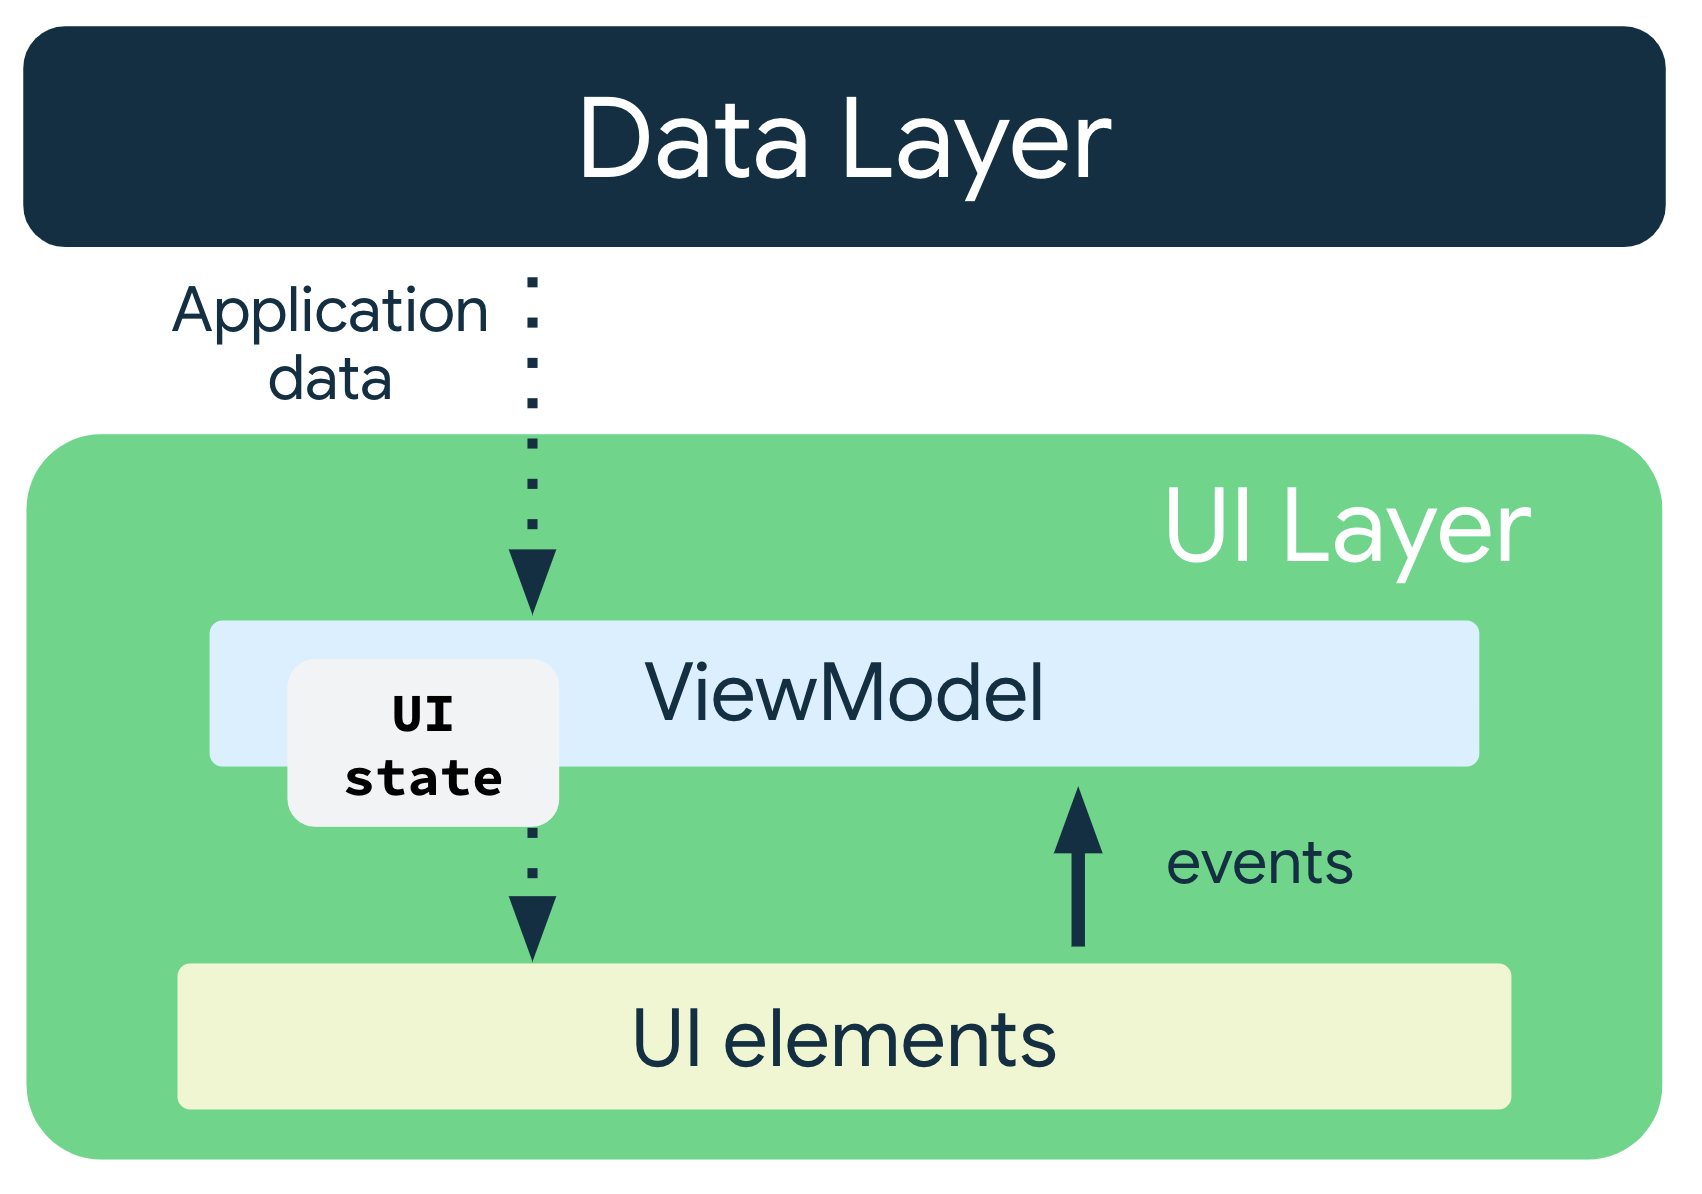
\includegraphics[width=.5\textwidth]{arch-ui-udf.png}
  \caption{Architektura UI vrstvy Zdroj: \cite{imgDataFlow}}
  \label{fig:arch_ui_udf}
\end{figure}

\myparagraph{ViewModel}
Hlavní účel ViewModelu je uchovávat a spravovat data potřebná pro zobrazení na obrazovce a to i při změnách konfigurace zařízení 
(například při otočení obrazovky) \cite{viewModelOver}. ViewModel také poskytuje metody a události pro interakci s~daty jako je načítání dat z úložiště, 
jejich aktualizace a předávání událostí od uživatele zpět do aplikace. Na základě těchto událostí například aktualizuje stav uživatelského
rozhraní. % (UI elementů) nebo stavu 

\myparagraph{UI state} \label{UIStateParagraph}
UI state (stav uživatelského rozhraní) je část UI vrstvy, který popisuje aktuální stav a chování uživatelského 
rozhraní v~daném okamžiku \cite{andDocArch}. Tento stav může zahrnovat různé informace jako jsou aktuální hodnoty vstupních polí, stav vybraných prvků,
 aktuální zobrazené obrazovky nebo panely, stav animací a další.

UI state je důležitý pro udržování konzistence a interaktivity uživatelského rozhraní. Změny v~UI stavu mohou být způsobeny uživatelskými
interakcemi jako například kliknutím na tlačítko, zadáním textu do pole, rolováním seznamu nebo mohou být vyvolány událostmi v~aplikaci v případech 
jako je získání dat ze serveru nebo jakoukoliv změnou interního stavu aplikace. 

V~rámci frameworků, které k~tvorbě UI používají deklarativní způsob zápisu se často k~definice stavu a jeho vlivu na UI používá funkce 
na obrázku \ref{fig:UI_function}. Ta zjednodušeně popisuje výsledné uživatelské rozhraní, které je tvořeno na základě jeho stavu.

\begin{figure}[H]
  \centering
  
\includegraphics[width=.5\textwidth]{ui-equals-function-of-state.png}
  \caption{Reprezentace vztahu UI a stavu aplikace Zdroj: \cite{imgUIformula}}
  \label{fig:UI_function}
\end{figure}

Správa UI stavu je důležitou součástí vývoje aplikací s~uživatelským rozhraním a může být implementována pomocí různých technik a nástrojů.
Důležité je udržovat UI stav v~souladu s~interním stavem aplikace a zajistit jeho konzistenci a správnou aktualizaci v~reakci na uživatelské 
interakce a události v~aplikaci.

\myparagraph{UI Elements}
UI elements neboli prvky uživatelského rozhraní jsou komponenty tvořící vizuální část aplikace a umožňují uživatelům interagovat s~aplikací. \cite{andDocArch}
Tyto prvky zahrnují různé vizuální komponenty jako jsou tlačítka, textová pole, seznamy, obrázky, ikony, přepínače, posuvníky atd., díky nimž
se zobrazují data reprezentující aktuální stav aplikace nebo je pomocí nich tento stav měněn.

UI prvky jsou navrženy tak, aby poskytovaly uživatelům intuitivní způsob jak s~aplikací komunikovat a manipulovat. Každý prvek má své 
vlastnosti jako je velikost, barva, text, stav atd., které lze nastavit a upravovat pomocí kódu. Tyto prvky jsou pak umístěny na obrazovce 
podle určeného rozvržení (layout), které určuje jejich pozici a vzájemné uspořádání.

UI prvky jsou základními stavebními bloky uživatelského rozhraní a hrají klíčovou roli při vytváření uživatelsky přívětivé a atraktivní aplikace. 
Jejich vhodné použití a umístění má vliv na celkový uživatelský zážitek a efektivnost aplikace.

\myparagraph{UI Events}
Nejčastějším typem UI událostí jsou takzvané uživatelské události, které jsou generovány interakcí uživatele s~uživatelským rozhraním aplikace. \cite{UIEvents}
Patří k~nim například kliknutí myší, dotyk na obrazovce, stisknutí klávesy nebo jakékoliv jiné akce prováděné uživatelem, které vyvolávají reakci
v~UI aplikaci.

O~zpracování uživatelských událostí se většinou stará příslušný ViewModel, který nabízí veškeré funkce, které je pomocí uživatelského rozhraní možné volat.
Nicméně, některé typy uživatelských událostí může UI zpracovat přímo. Takovými událostmi jsou například navigování na jinou obrazovku nebo zobrazení 
informativní zprávy pomocí takzvaných \textit{Snackbars}.

\subsection*{Doménová vrstva}
Doménová vrstva typicky obsahuje způsoby užití. Nicméně, pro menší aplikace jako je tato, může být vynechána. \cite{domainLayerAnd} Často se tímto 
způsobem \uv{odlehčují} ViewModely, které by jinak obsahovaly příliš mnoho kódu, což by vedlo k~nepřehlednosti.

V~tomto projektu doménová vrstva zahrnuje deklarace výčtových typů, objektů pro datovou a modelovou vrstvu a mapovací funkce pro převod
objektů datové vrstvy na objekty používané v~prezentační vrstvě a naopak.

Doménová vrstva by měla být nezávislá na technických aspektech aplikace a měla by se zaměřovat pouze na reprezentaci a správu doménových
 konceptů a procesů.\cite{ssw} To zjednodušuje testování, údržbu, rozšiřitelnost aplikace a umožňuje snadnou změnu technologií nebo platformy bez 
 vlivu na doménovou logiku. 

\subsection*{Datová vrstva}
%Datová vrstva se stará o správu dat, která mohou být aplikaci poskytnuta například uživatelem nebo nějakou externí službou.
%he data layer that contains the business logic of your app and exposes application data.


Datová vrstva se stará o persistenci dat a komunikaci s~datovými úložišti jako jsou
databáze, soubory nebo vzdálené API. Jejím hlavním úkolem je poskytovat rozhraní mezi doménovou logikou aplikace a datovými zdroji, 
aby bylo možné ukládat, načítat, aktualizovat a mazat data podle potřeby. \cite{datalayer}

K~tomu aby aplikace fungovala, jak bylo popsáno v~úvodu této kapitoly, je zapotřebí, aby datová vrstva implementované aplikace obsahovala mechanismy pro
 získání dat z~informačních systémů města a vhodně je kombinovala s daty uloženými v lokální databázi.
 
Jelikož se data v~informačních systémech města nachází ve formátu XML, byla proto navržena služba získávající tato data ze vzdáleného 
datového zdroje (IS města) způsobem zobrazeným v~levé části obrázku \ref{fig:arch_data_layer}. Získaná data jsou následně propojena s aplikací
pomocí takzvaných \textit{Data access object}, jejichž princip je podrobněji popsán dále v této sekci.

Pro persistenci těchto dat byla vybrána SQL databáze založená na enginu SQLite, která se stará o poskytnutí dříve načtených dat 
v~případech, kdy aplikace nemá přístup k~internetu.


\begin{figure}[H]
  \centering
  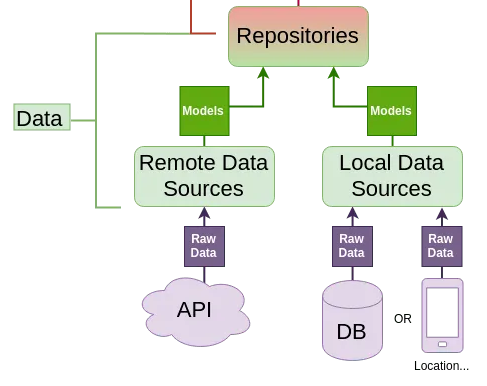
\includegraphics[width=.5\textwidth]{data_layer_diagram.png}
  \caption{Architektura datové vrstvy Zdroj: \cite{imgDataFlow}}
  \label{fig:arch_data_layer}
\end{figure}

% \begin{figure}[H]
%   \centering
%   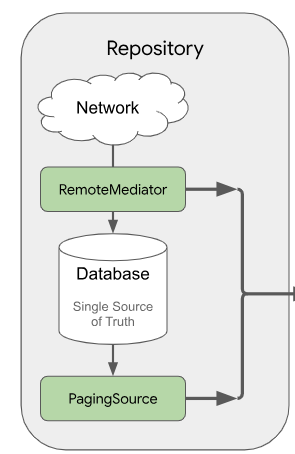
\includegraphics[width=.3\textwidth]{data_layer_diagram_principle.png}
%   \caption{Architektura datové vrstvy}
%   \label{fig:arch_data_layer_principle}
% \end{figure}

Následující výčet prvků má za úkol představit důležité komponenty datové vrstvy používané v rámci navržené aplikace.

\myparagraph{Data access object}
Data access objects (zkráceně \textit{DAOs}) jsou zodpovědné za přímý přístup k~datovým úložištím a provádění operací jako čtení, zápis, aktualizace a mazání dat. \cite{oracleDAO} Tyto objekty 
poskytují abstrakci nad konkrétními technologiemi datových úložišť a umožňují snadnou změnu úložišť bez vlivu na ostatní části aplikace.

V rámci navržené aplikace jsou navržené pro přistup do lokální databáze. 

\myparagraph{Data transfer object}
Data transfer object (zkráceně \textit{DTO}) jsou objekty používané k~přenosu dat mezi vrstvami aplikace. Tyto objekty slouží k~přenosu dat mezi datovou vrstvou a doménovou 
vrstvou a často mapují datové entity na jednodušší objekty nebo struktury pro snadnější manipulaci. \cite{DTO}
Jak již bylo zmíněno dříve, tak DTOs jsou navrženy v procesu získávání dat z informačních systémů města a slouží k převodu XML dat, získaných
ze serveru města.   

\myparagraph{Datové entity}
Datové entity představují strukturu a schéma dat uložených v~databázi nebo jiném datovém úložišti. Tyto entity obvykle přímo odrážejí
strukturu tabulek v~relační databázi nebo dokumentů v~NoSQL databázi a poskytují model, se kterým mohou pracovat ostatní vrstvy aplikace.

\myparagraph{Datová úložiště}
Datová úložiště jsou fyzická místa, kde jsou data uložena. Mohou to být relační databáze, NoSQL databáze, soubory na disku nebo externí API. 
Datová vrstva zajišťuje, aby bylo možné efektivně pracovat s~těmito úložišti, a zároveň byla data bezpečně uložena a získána.

\bigskip

Poslední tři zmíněné části jsou pak v rámci navržené datové vrstvy propojeny následujícím způsobem:

\begin{figure}[H]
  \centering
  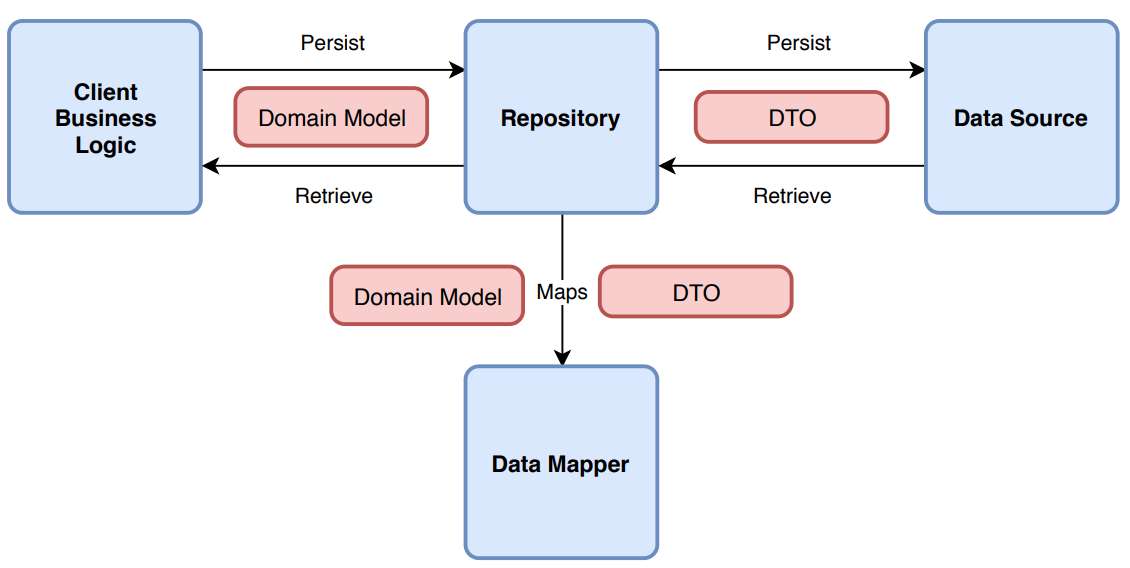
\includegraphics[width=.8\textwidth]{arch_diagram.png}
  \caption{Provázanost jednotlivých částí datové vrstvy Zdroj: \cite{imgDataDiagram}}
  \label{fig:arch_diagram}
\end{figure}


% \dirtree{%
%         .1 src \DTcomment{}.
%           .2 androidMain \DTcomment{}.
%           .2 commonMain \DTcomment{je pro kód sdílený mezi všemi platformami}.
%             .3 kotlin \DTcomment{}.
%               .4 data\DTcomment{datová vrstva}.
% 		            .5 model\DTcomment{}.
% 		            .5 repository.
% 		          .4 ui\DTcomment{prezentační vrstva}.
% 		            .5 composables\DTcomment{}.
% 		            .5 screens\DTcomment{}.
% 		              .6 HomeScreen\DTcomment{}.
%             .3 resourses \DTcomment{}.
%           .2 desktop Main \DTcomment{}.
% 	}


% \begin{figure}[H]
%   \centering
%   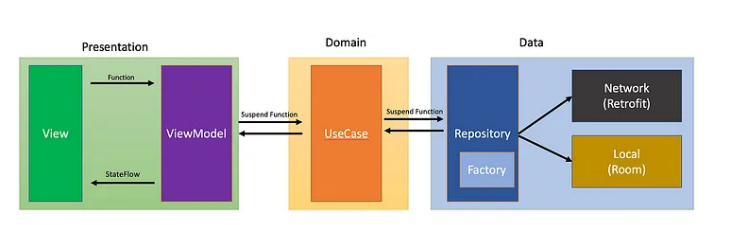
\includegraphics[width=1\textwidth]{mvvm.png}
%   \caption{MVVM with Clean Architecture}
%   \label{fig:mvvm}
% \end{figure}

\section{Uživatelské rozhraní}
% UI bylo navrhováno tak aby vyhovovalo TODO

% v~Android dokumentaci jejíž části se zaměřují na návrh od jednotlivých tlačítek, textů až po to, jak celé UI působí z~pohledu
% uspořádání.



% TODO pravidla stravneho navrhu UI

\subsection{Drátěné modely} \label{navrhWireframes}
% K~tomu, aby bylo výsledné UI pro uživatele přívětivé, bylo přistupováno tak, aby co nejvíce korespondovalo s~pravidly dobrého návrhu UI.

% Mezi taková pravidla patří:
% TODO

Navržené drátěné modely byly vytvořeny na základě funkčních požadavků a to tak, aby nejdůležitější a nejčastěji používané funkce byly 
umístěny na domovskou obrazovku. Zbylé méně podstatné nebo prostorově náročnější byly umístěny na sekundární obrazovky.



\pagebreak
\begin{minipage}[t]{0.45\textwidth}
  
  \myparagraph{Obrazovka \textit{Domů}\medskip}
  %Jak již bylo zmíněno v úvodu této kapitoly, tak 
  Obrazovka \textit{Domů} (viz obrázek \ref{fig:wireframe1}) byla navržena tak, aby jakožto hlavní stránka celé aplikace obsahovala pro uživatele
  co nejpřínosnější informace a zároveň, aby sloužila jako určitý rozcestník na další obrazovky aplikace. Z~tohoto důvodu byla do horní části obrazovky
  navržena tlačítka, která uživateli umožňují rychlý prostup na YouTube kanál města, nahlášení závady, zobrazení úředních hodin nebo stránku služeb města.
  
  %Na základně...byla pro události vybrána možnost zobrazení jednotlivých událostí
  \smallskip
  Do střední části obrazovky byl navržen posuvný řádek obsahující nově přidané události a to především díky možnosti zobrazit
  veškeré potřebné události kompaktně na malém prostoru, ale přesto uživateli nabídnout možnost danou událost otevřít a dohledat zbylé informace.
  Události tak na sebe poutají největší pozornost především svou vizuální reprezentací a převážná část informace je uživateli předána právě pomocí titulního obrázku, názvu
  a času konání.
  
  \smallskip

  Oproti tomu pro seznam novinek ve spodní části obrazovky bylo vybráno uspořádání novinek do posuvného sloupce. Ten lépe umožňuje 
  využít celou šíři obrazovky k~zobrazení delších titulků a textů, které jsou pro uživatele v~případě aktualit nejdůležitější.
  
  
  \bigskip
  \myparagraph{Obrazovka \textit{Události}\medskip}
  V~rámci obrazovky \textit{Události} (viz obrázek \ref{fig:wireframe2}) je použit stejný systém pro zobrazení událostí - pomocí posuvného řádku, 
  stejný způsob je použit na obrazovce \textit{Domů}.
  \smallskip
  
  Oproti domovské stránce jsou zde však zobrazeny veškeré události, které se ve městě budou konat. Pro lepší přehled jsou události rozděleny 
  do několika kategorií jako například \textit{Kino}, \textit{Divadlo}, \textit{Celodenní akce}, \textit{Akce pro děti} nebo \textit{Přednášky}.
  
  V~horní části aplikace je pak uživateli dána možnost vybrat den, pro který chce zobrazit plánované události a případně si zvolit požadované rozmezí.
  \smallskip

  To je možné navolit pomocí kalendáře, který se zobrazí po kliknutí na ikonu kalendáře v~pravé horní části obrazovky.
  
  %
  
  
  Aplikace byla navržena tak, aby uživatelé mohli jednoduše filtrovat zobrazované události primárně podle času.
  

 
\end{minipage}
\hfill
\begin{minipage}[t]{0.45\textwidth}
  \begin{figure}[H]
    \centering
    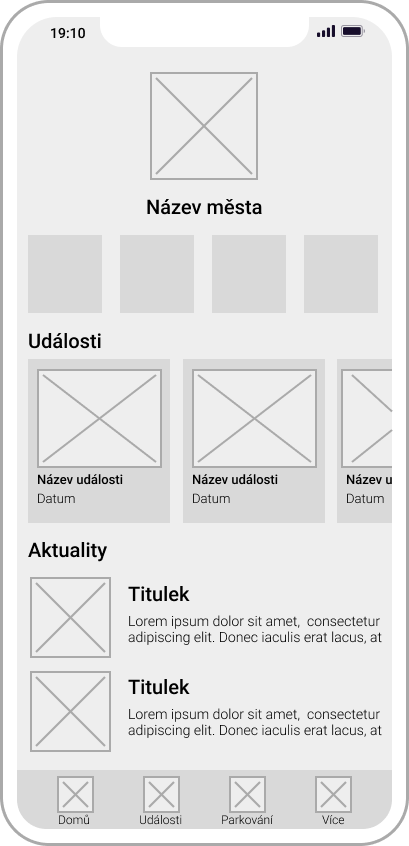
\includegraphics[width=.7\textwidth]{home_wireframe.png}
    \caption{Drátěný model obrazovky \textit{Domů}}
    \label{fig:wireframe1}
  \end{figure}
  \begin{figure}[H]
    \centering
    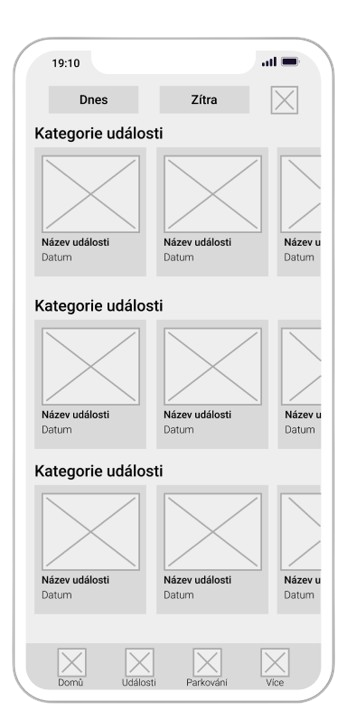
\includegraphics[width=.7\textwidth]{events_wireframe.png}
    \caption{Drátěný model obrazovky \textit{Události}}
    \label{fig:wireframe2}
  \end{figure}
\end{minipage}

\begin{minipage}[t]{0.45\textwidth}
  Filtrování podle kategorie bylo nejprve navrženo, ale následně od něho bylo upuštěno kvůli malému počtu kategorií.
  
  Ve finále byl tedy zvolen přístup, který vybrané události přiřadí do patřičné kategorie a zobrazí jen ty kategorie, které obsahují alespoň jednu událost.

\myparagraph{Obrazovka \textit{Parkování}\medskip}
Obrazovka parkovaní (viz obrázek \ref{fig:wireframe3}) slouží uživateli dle dříve specifikovaných případů užití, především k~vyhledání parkovací zóny, 
získání informací o~ceně parkování a případně k~platbě parkovacích poplatků. Z~těchto důvodů byla hlavní část obrazovky věnována mapovému podkladu, 
který uživateli umožňuje snadné nalezení parkovací zóny v~mapě města. % jehož součástí je množina parkovacích zón.

\smallskip
% Aby bylo docíleno co nejjednodušší manipulace s mapovými podklady byl prostor obrazovky navržen tak aby hlavní část byla věnována právě mapovému
% podkladu na němž jsou vyznačeny parkovací zóny. 

Pro ještě snadnější hledání parkovacích zón dává aplikace uživateli možnost vyhledání požadované parkovací zóny pomocí vyhledávacího pole, které umožňuje vyhledat příslušnou parkovací zónu buďto podle čísla nebo názvu zóny. 

\smallskip

Dále zde byla implementována výsuvná karta ze spodní části obrazovky, která se zobrazí pouze v~případě, že uživatel vybere jednu
z~nabízených parkovacích zón. Díky této implementaci se uživateli nezmenšuje prostor pro rychlé vyhledání parkovací zóny,
které je hlavním cílem k~použití této obrazovky. 
\smallskip
Tato výsuvná karta uživateli zobrazí detailní informace k~vybrané parkovací zóně a umožní zaplatit parkovací poplatek pro vybranou parkovací zónu.

\smallskip

Poslední funkcí, kterou tato obrazovka nabízí je zobrazení aktuální dopravní situace ve městě, která je na mapě zobrazena spolu s~parkovacími zónami.

\medskip

\myparagraph{Obrazovka \textit{více}\smallskip}
Poslední navrženou obrazovkou je obrazovka \textit{Více} (viz obrázek \ref{fig:wireframe4}), která obsahuje přehled veškerých méně podstatných částí aplikace.

%Jelikož je ale aplikace cílena pro široké spektrum lidí, byl zde navržena funkce, která umožňuje přidání vybraného prvku na domovskou obrazovku.


%který uživatelům umožňuje přízpůsobení domovské obrazovky.
%při dlouhém stisknnutí zobrazí možnost přidání prvku na domovskou obrazovku.
%které mohou být přidány na uvodní obrzovku.


%v případě, že by uživatel shledal některou 
%z nabízených funkcí důležitější/častěji potřebnou, tak umožňuje uživateli tuto funkci přidat na domovskou obrazovku.

%Představuje rychlo navigaci

%Obsahuj důležité prvky aplikace, které obsahují veškeré méně podstatné části aplikace.
\end{minipage}
\hfill
\begin{minipage}[t]{0.45\textwidth}
  \begin{figure}[H]
    \centering
    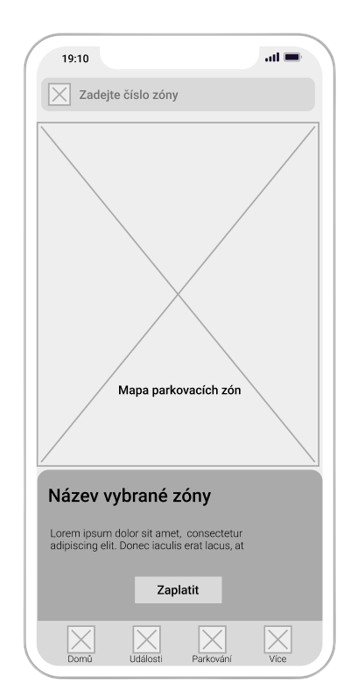
\includegraphics[width=.7\textwidth]{parking_wireframe.png}
    \caption{Drátěný model obrazovky \textit{Parkování}}
    \label{fig:wireframe3}
  \end{figure}
  \begin{figure}[H]
    \centering
    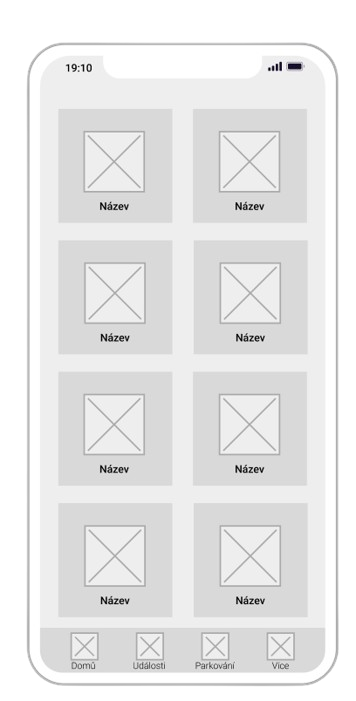
\includegraphics[width=.7\textwidth]{more_wireframe.png}
    \caption{Drátěný model obrazovky \textit{Více}}
    \label{fig:wireframe4}
  \end{figure}
\end{minipage}

\subsection{Design systém} \label{designSystemSection}
Před tím něž bylo přistoupeno ke grafickému návrhu aplikace, tak byl vytvořen obecný design systém, který poslouží k~vytvoření 
konzistentního uživatelského rozhraní. Zároveň se díky němu urychlí proces navrhovaní grafické podoby UI a při následné fázi implementace 
zajistí intuitivní ovládání aplikace na všech implementovaných platformách. 

%Design system je obecně vzato sada komponent, pravidel, principů a návrhových postupů, které slouží k vytváření konzistentního
%uživatelského rozhraní a uživatelského zážitku napříč různými aplikacemi a platformami. 

Design systém je obecně vzato sada předem definovaných pravidel, komponent, standardů a návrhových principů, které slouží k~vytváření a udržování 
konzistentního a jednotného vizuálního stylu v~rámci celé aplikace \cite{ds}. Takový systém zahrnuje různé prvky jako jsou barvy, typografie, ikony,
způsoby rozložení UI nebo komponenty uživatelského rozhraní a umožňuje vývojářům a designérům efektivně spolupracovat a vytvářet aplikace s~jednotným 
vzhledem. 

Cílem návrhu design systému je zajistit, aby všechny části aplikace měly jednotný vzhled a chování, což zlepšuje především uživatelskou 
zkušenost s~danou aplikací. 
%Designový systém zároveň často obsahuje sadu prvků UI, typografického stylu, barev, ikon a další informace, které 
%pomáhají designérům a vývojářům při tvorbě aplikací.

%V navrhovaní výsledného design systému bylo přistupováno tak aby styl navržených UI komponenty, typů písma, barem a dalších prvků design 
%systému přibližně odpovídal aktuálně používanému stylu města.

%Jelikož město, které bylo vybráno pro implementaci aplikace nikde explicitně nedefinovalo používaný design systém,
%byl proto vytvořen na základě.  
%TODO NEBO 

V~rámci vybraného města Příbrami není takový systém nikde explicitně zadefinovaný, a proto byl odvozen z~designu webových stránek města.
%pro navození maximálního pocitu jednoty s dosavadními informačními systémy města.
Zároveň byl zkombinovaný s~aktuálně nejnovějším design systémem od společnosti Google zvaným \textit{Material Design 3} \cite{m3d}.
%, který je vhodný nejen pro použití na mobilních platformách.

S~ohledem na to, že aplikace je navrhována pro použití na mobilních zařízeních, tak je tomu uzpůsoben i návrh samotného design systému, který
specifikuje především barvy, styly textů a prvky použitelné na mobilních platformách. Zbylé části mohou být případně v~budoucnu rozšířeny o~další prvky 
používané na jiných platformách.

Součástí návrhu je tak několik základních UI prvků, které budou použity v~rámci implementované aplikace a mohou být použity i případně dalšími 
aplikacemi města.

Výsledek základní ukázky takto navrženého systému je k~vidění na obrázku \ref{fig:design_system}

\bigskip

\begin{figure}[H]
  \centering
  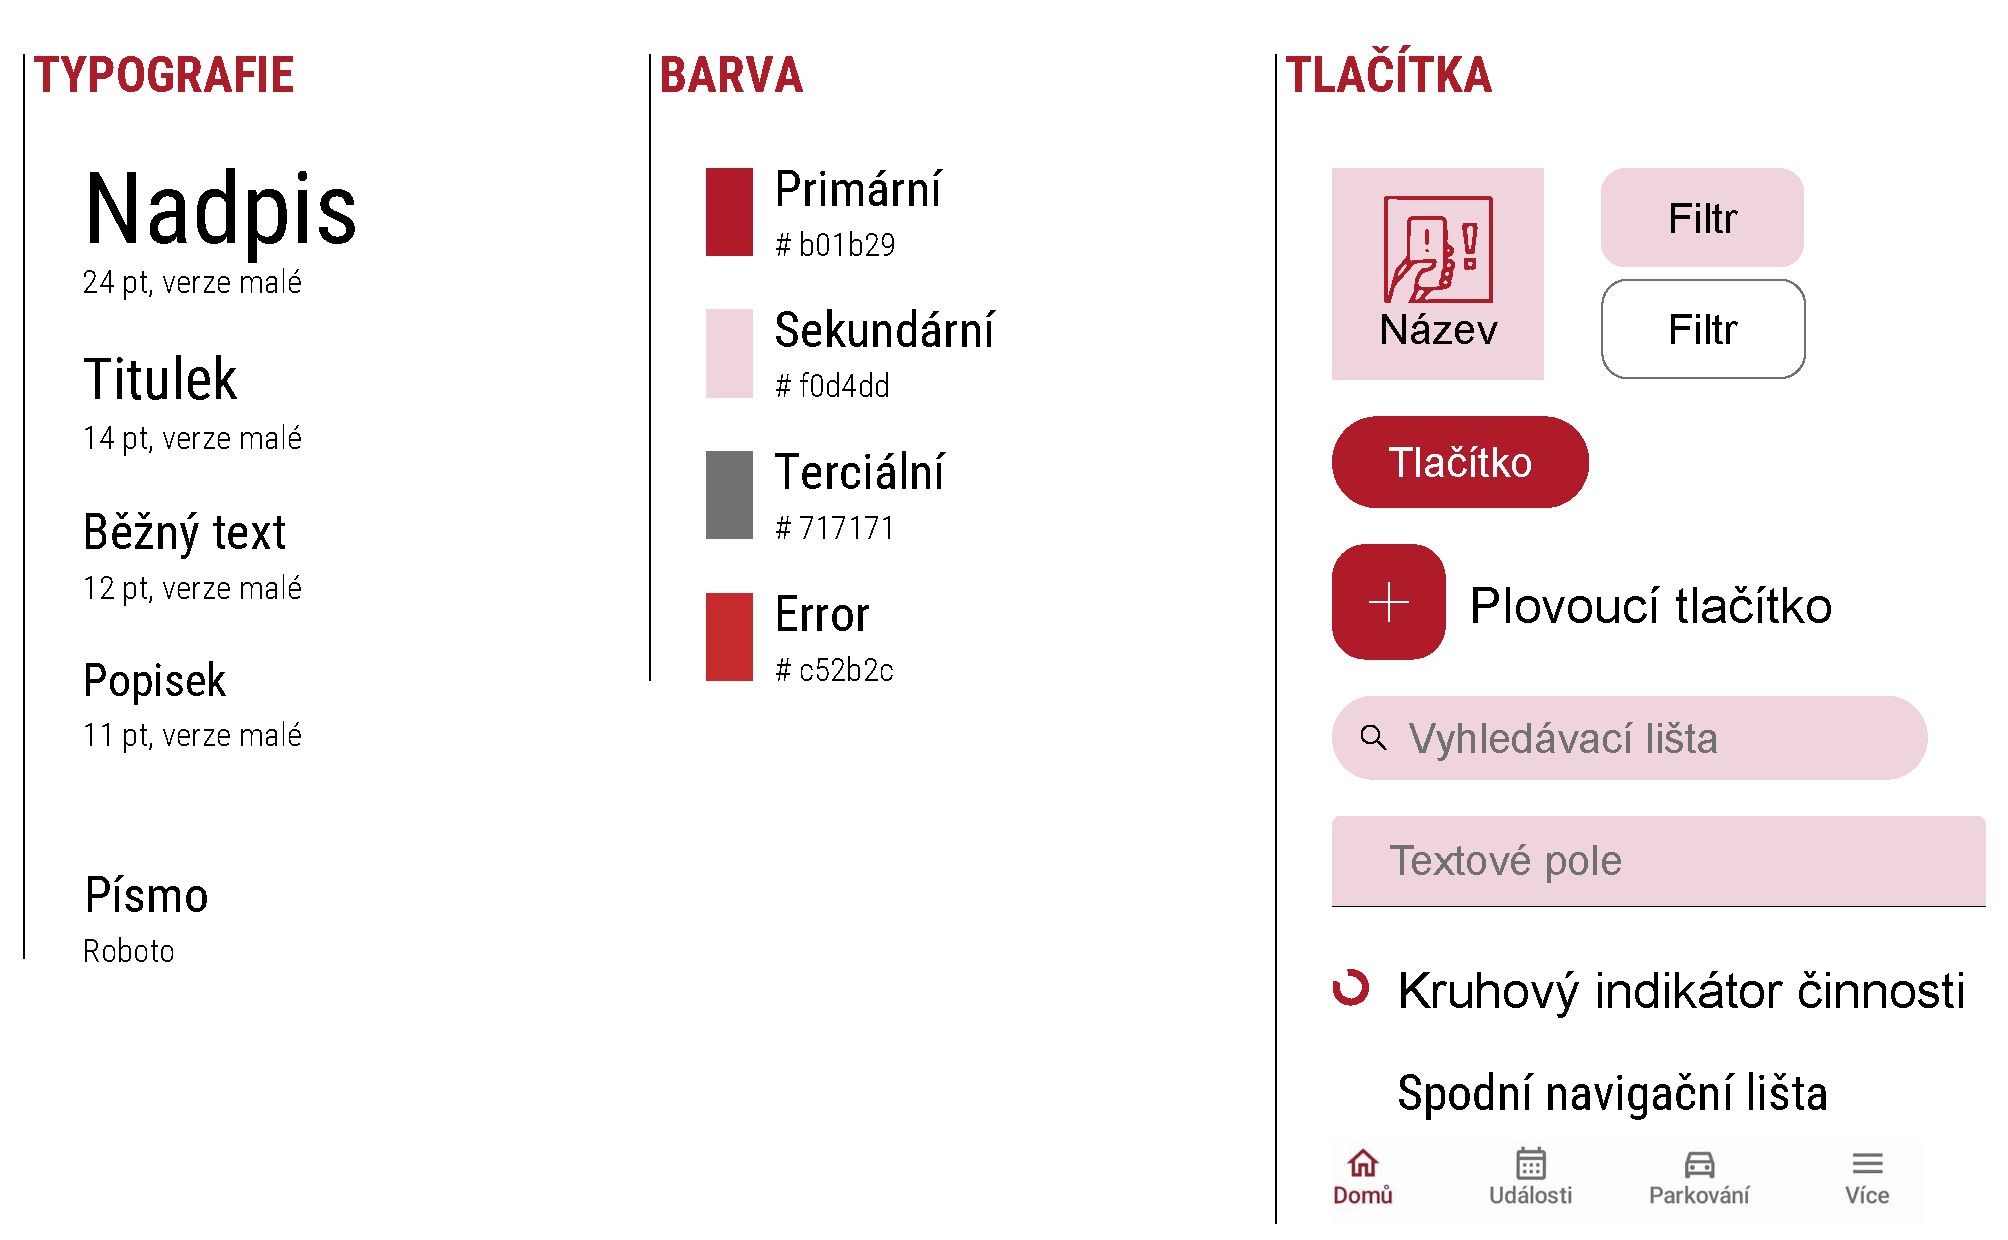
\includegraphics[width=.99\textwidth]{design_system.jpg}
  \caption{Ukázka navrženého design systému}
  \label{fig:design_system}
\end{figure}

\subsection{Mockup modely} \label{navrhMockupModelu}
Po zadefinování použitelných komponent v~předchozí sekci \textit{Design systém \ref{designSystemSection}} 
je již samotný návrh grafické podoby uživatelského rozhraní zjednodušen na nezbytné minimum. Vytvořené mockup modely jsou totiž de facto výsledkem sloučení drátěných modelů
 s~navrženým design systémem.

Při návrhu grafické podoby UI byla proto pozornost primárně soustředěna na význam jednotlivých UI komponent a na základě jejich významu byly
přiřazovány například odpovídající barvy. 

Navržené uživatelské rozhraní se tímto přístupem snaží respektovat zásady správného UI návrhu dle Android dokumentace 
a to především z~pohledu přístupnosti, rozložení obsahu, druhu použitých UI komponent nebo vhodnosti použití barev z~hlediska sémantiky barev.

%\pagebreak
\begin{minipage}[t]{0.45\textwidth}

\bigskip
\myparagraph{Přístupnoust\medskip}
Z~hlediska přístupnosti je uživatelské rozhraní aplikace navrženo tak, aby jednotlivé prvky UI měly vhodně zvolenou barvu z~pohledu
správného kontrastu vůči podkladu anebo z~pohledu dostatečné čitelnosti.

\smallskip

Dále byla věnována pozornost správnému popisu jednotlivých UI komponent a správnému použití dle druhu komponenty tak, aby bylo možné aplikaci používat i
s~takzvanou TalkBack čtečkou, která umožňuje nevidomým nebo jinak zrakově postiženým lidem používat aplikaci například na základě hlasové odezvy.

\bigskip
\myparagraph{Barvy\medskip}
I~přesto, že základní barvy byly zvoleny již při navrhování design systému, během fáze návrhu mockup modelu byl kladen důraz na jejich 
vhodné použití a to především z~pohledu sémantiky barev nebo důležitosti barvených komponent.

\smallskip
%je barva primárním, sekundárním  ternární navržené v rámci designs sytému

Základní popisy barev použité při návrhu design systému byly odvozeny z~\textit{Material 3} design systému, v~rámci kterého mají jasně 
vymezené role. \cite{m3ColorRoles}
Primární barva je proto v~případě implementovaného UI například použita pro potvrzovací akci \uv{zaplacení parkovacích poplatků}. 
Sekundární barva byla naopak
implementována například na filtrační tlačítka na obrazovce \textit{Události}, jelikož hlavním předmětem pozornosti na dané obrazovce 
jsou zobrazované akce a nikoliv filtrační možnosti.

\bigskip



 %Sytost barev byla zvolena na základě
\end{minipage}
\hfill
\begin{minipage}[t]{0.45\textwidth}
  \begin{figure}[H]
    \centering
    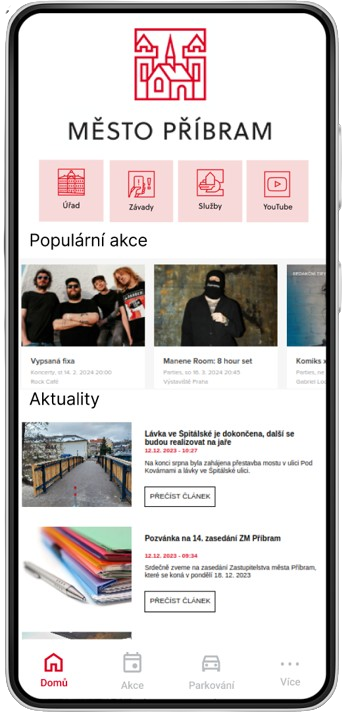
\includegraphics[width=.7\textwidth]{screen1.png}
    \caption{Obrazovka \textit{Domů}}
    \label{fig:mockup1}
  \end{figure}
  \begin{figure}[H]
    \centering
    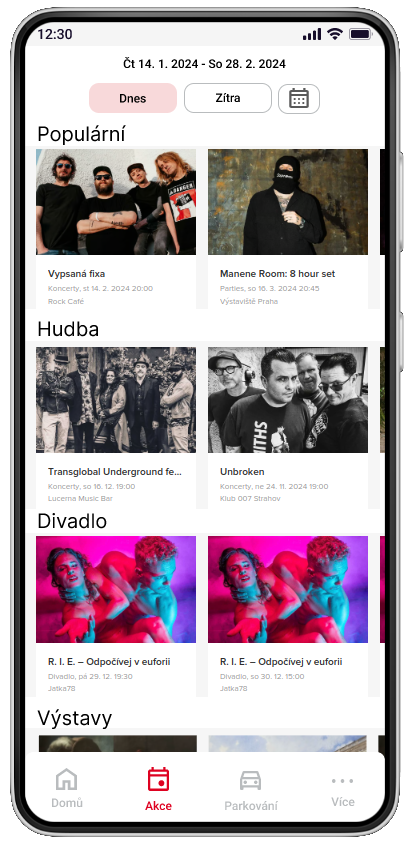
\includegraphics[width=.7\textwidth]{screen2.png}
    \caption{Obrazovka \textit{Události}}
    \label{fig:mockup2}
  \end{figure}
\end{minipage}

\pagebreak

\begin{minipage}[t]{0.45\textwidth}
  \myparagraph{Rozložení\medskip}
  Co se rozložení UI komponent na obrazovky týká, tak zde bylo respektováno několik pravidel, jako například liniového zarovnání UI komponent tak,
   aby nedocházelo k~narušení čitelnosti nebo dodržení minimální vzdálenosti od krajů obrazovky při umísťování důležitých UI komponent.
  
\smallskip

  Komponenty jako primární navigace nebo tlačítka, která slouží pro vykonávání důležitých akcí byla implementována na taková místa, 
  aby byla v~takzvané dosahové vzdálenosti.
  
  \smallskip

  Pro obrázky byly voleny běžné poměry jako například 4:3, aby nedocházelo k~jejich zbytečnému ořezávání.
\end{minipage}
\hfill
\begin{minipage}[t]{0.45\textwidth}
  \begin{figure}[H]
    \centering
    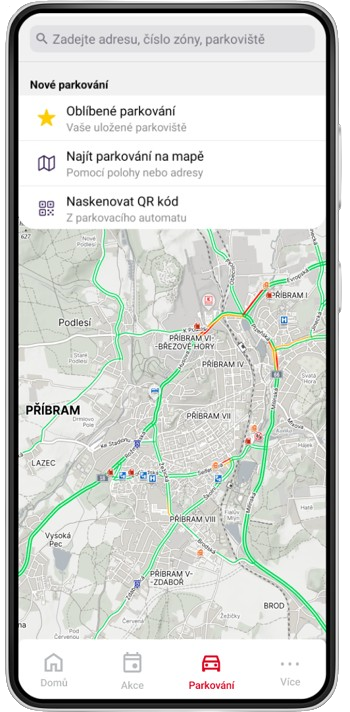
\includegraphics[width=.7\textwidth]{screen3.png}
    \caption{Obrazovka \textit{Parkování}}
    \label{fig:mockup3}
  \end{figure}
  \begin{figure}[H]
    \centering
    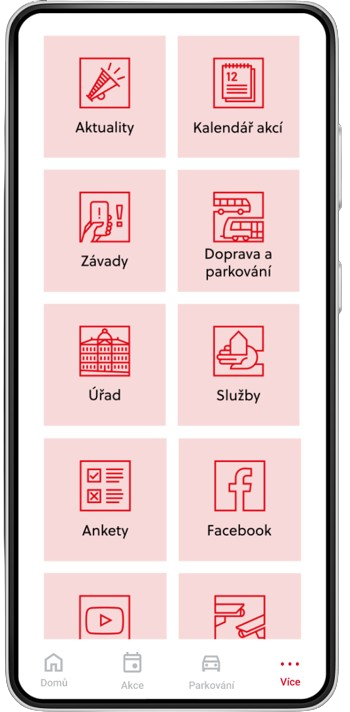
\includegraphics[width=.7\textwidth]{screen4.png}
    \caption{Obrazovka \textit{Více}}
    \label{fig:mockup4}
  \end{figure}
\end{minipage}
